\subsection{Cinemàtica inversa}

El càlcul invers és el que ens serveix per trobar els angles a partir de la posició a la que volem situar la plataforma. Es pot fer el càlcul per cada motor de manera separada. Primer s'han de definir les mides principals del robot que s'utilitzaran en el càlcul.

\subsubsection{Definicions de variables}
\begin{figure}[h!]
\centering
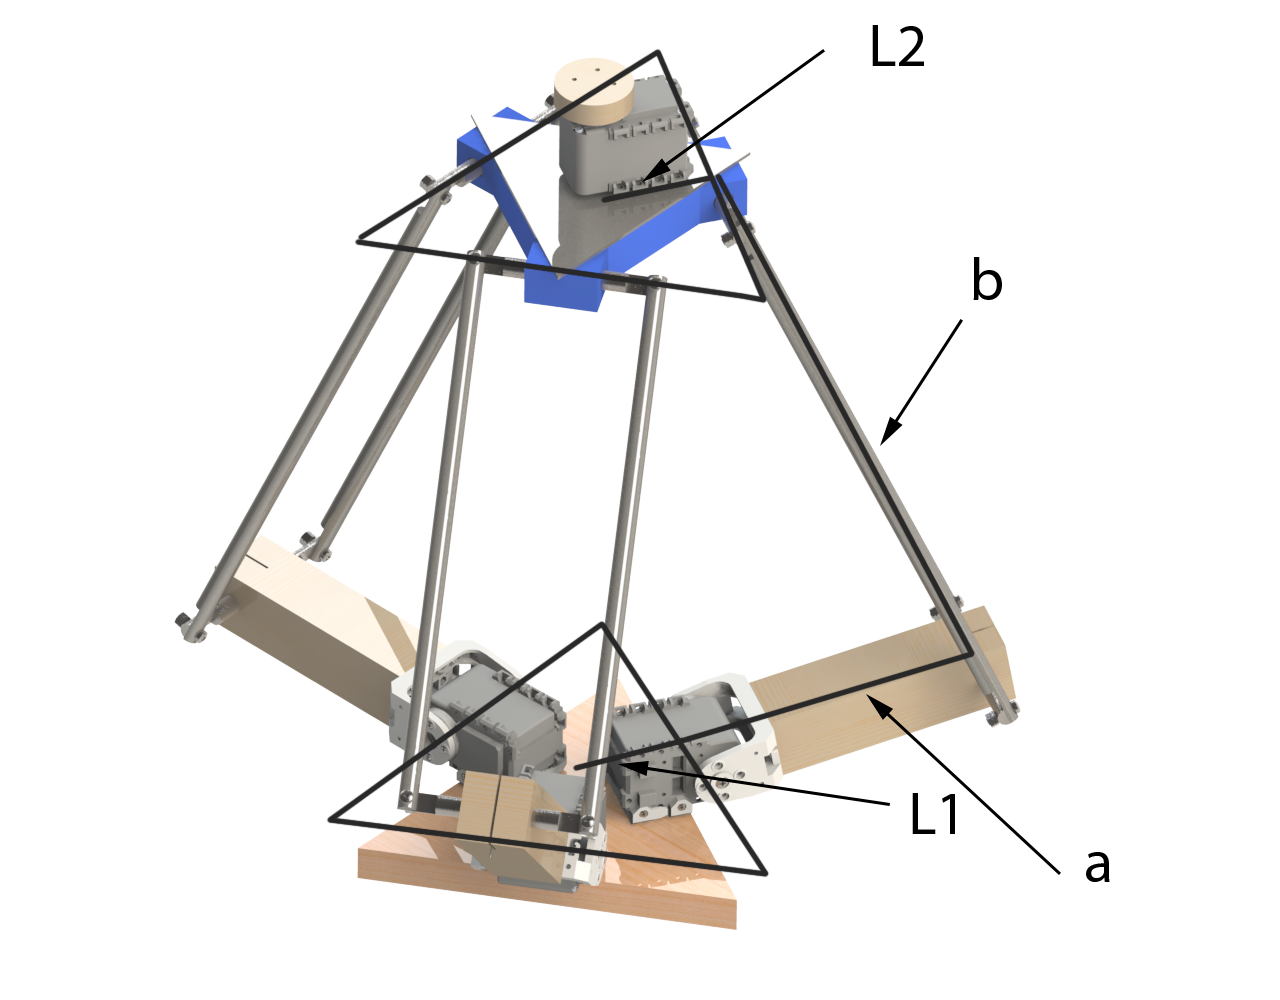
\includegraphics[width=12cm]{./imgComp/esquema_general}
\end{figure}

\begin{description}
\item[a] és la mida total del braç, des de l'eix del motor fins a l'eix de la connexió amb l'avantbraç.
\item[b] és la mida de tot l'avantbraç des de la connexió amb el braç fins a la unió amb la plataforma.
\item[L1] és la distància entre el centre de la base als eixos dels motors.
\item[L2] és la distància entre el centre de la plataforma a l'eix de connexió amb l'avantbraç.
\end{description}

\subsubsection{Canvis de base}
Com el càlcul de cada angle es independent de la resta, es poden fer canvis de base per poder fer-ho tot amb una sola funció a l'hora de programar. La base inicial \(\{x_0,y_0,z_0\}\) esta al centre de la base, amb la x en la direcció del motor 1. Les bases \(\{x_i,y_i,z_i\}\) que farem servir per calcular l'angle del motor \emph{i} estan posicionades al centre del eix de cada motor, i la seva x apunta en la direcció perpendicular al eix del motor. També es suma L2 a \(x_i\) per fer que la posició objectiu sigui el punt de connexió entre la plataforma i l'avantbraç en lloc del centre de la plataforma.

\begin{figure}[h!]
\centering
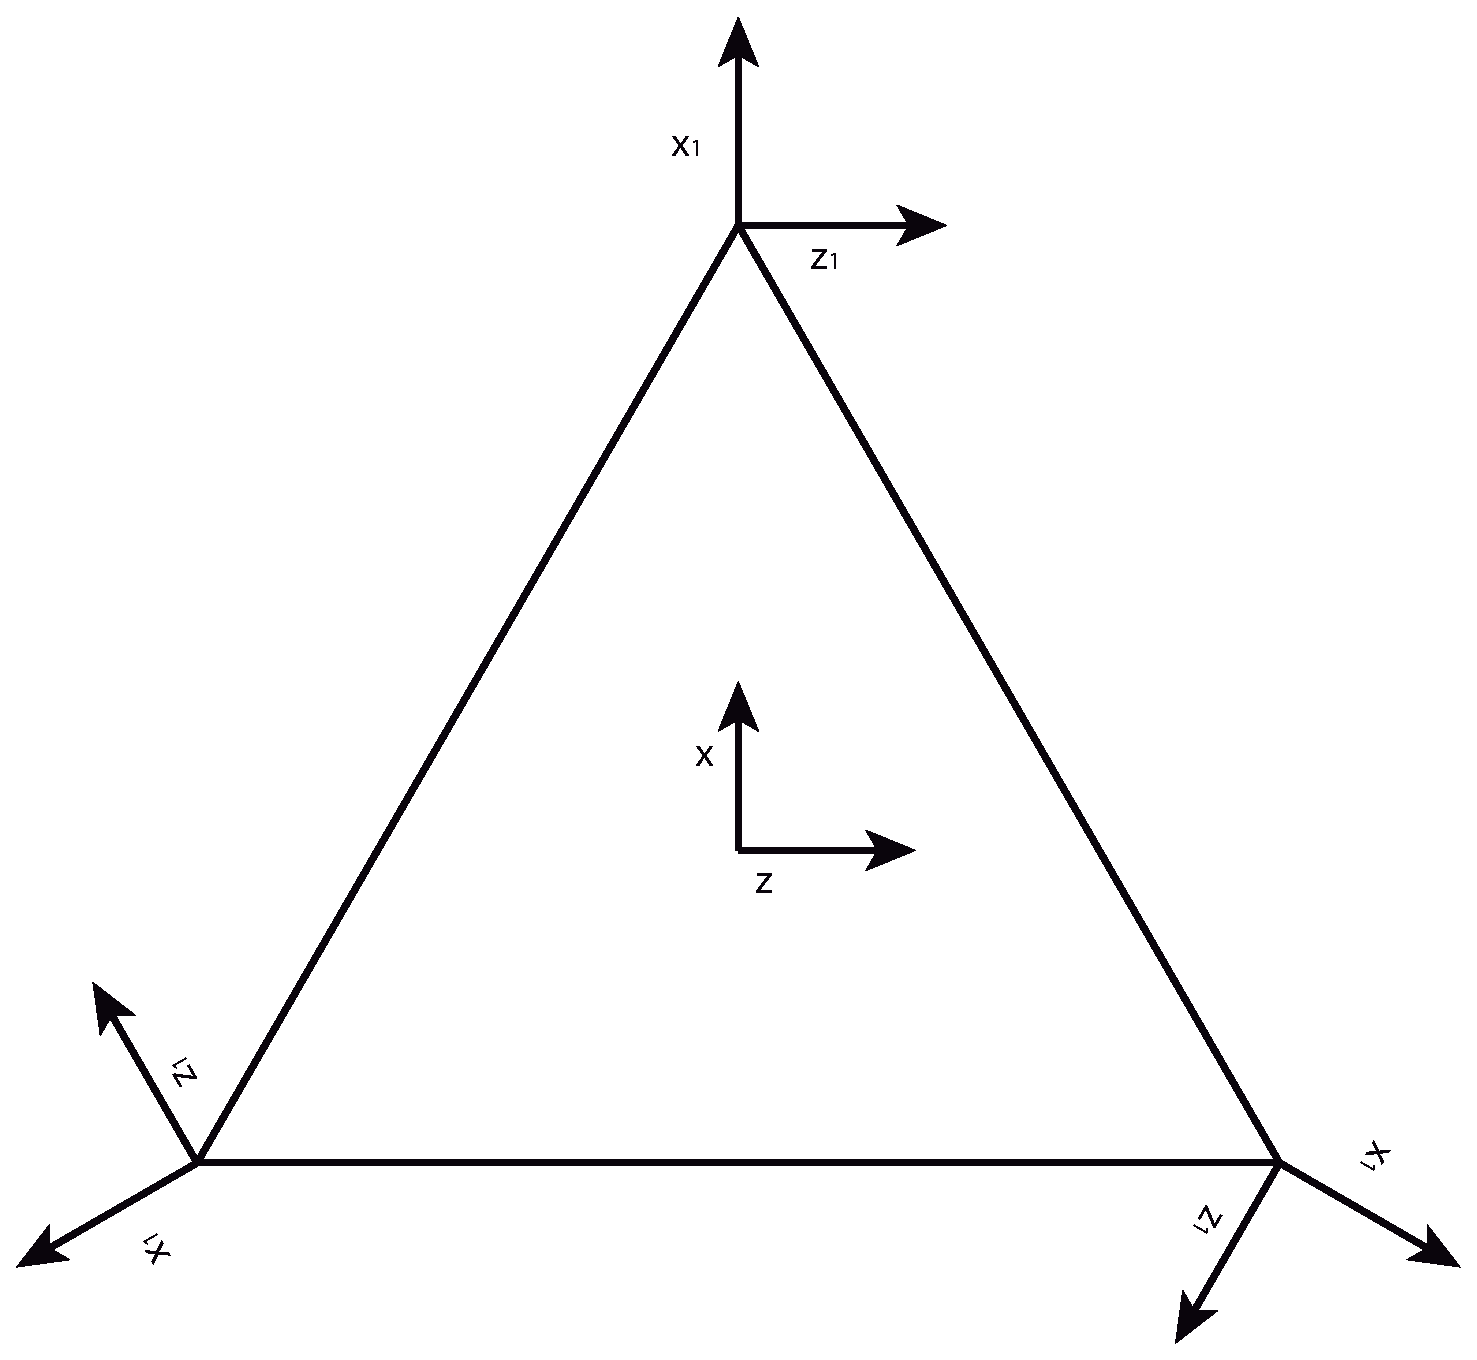
\includegraphics[width=7cm]{./sketch/canvi_base}
\end{figure}

\[\{x_1,y_1,z_1\}=\{x_0+L2-L1,y_0,z_0\}\]
\[\{x_2,y_2,z_2\}=\{z_0sin(60)-x_0cos(60)+L2-L1,y_0,-z_0cos(60)-x_0sin(60)\}\]
\[\{x_3,y_3,z_3\}=\{-z_0sin(60)-x_0cos(60)+L2-L1,y_0,-z_0cos(60)+x_0sin(60)\}\]

\subsubsection{Càlcul d'un angle}

El motor només pot moure el final del braç en un cercle, gràcies a això es poden deduir dos formules:\[x^2+y^2=a^2 \quad \textrm{i} \quad z=0\]

\begin{figure}[h!]
\centering
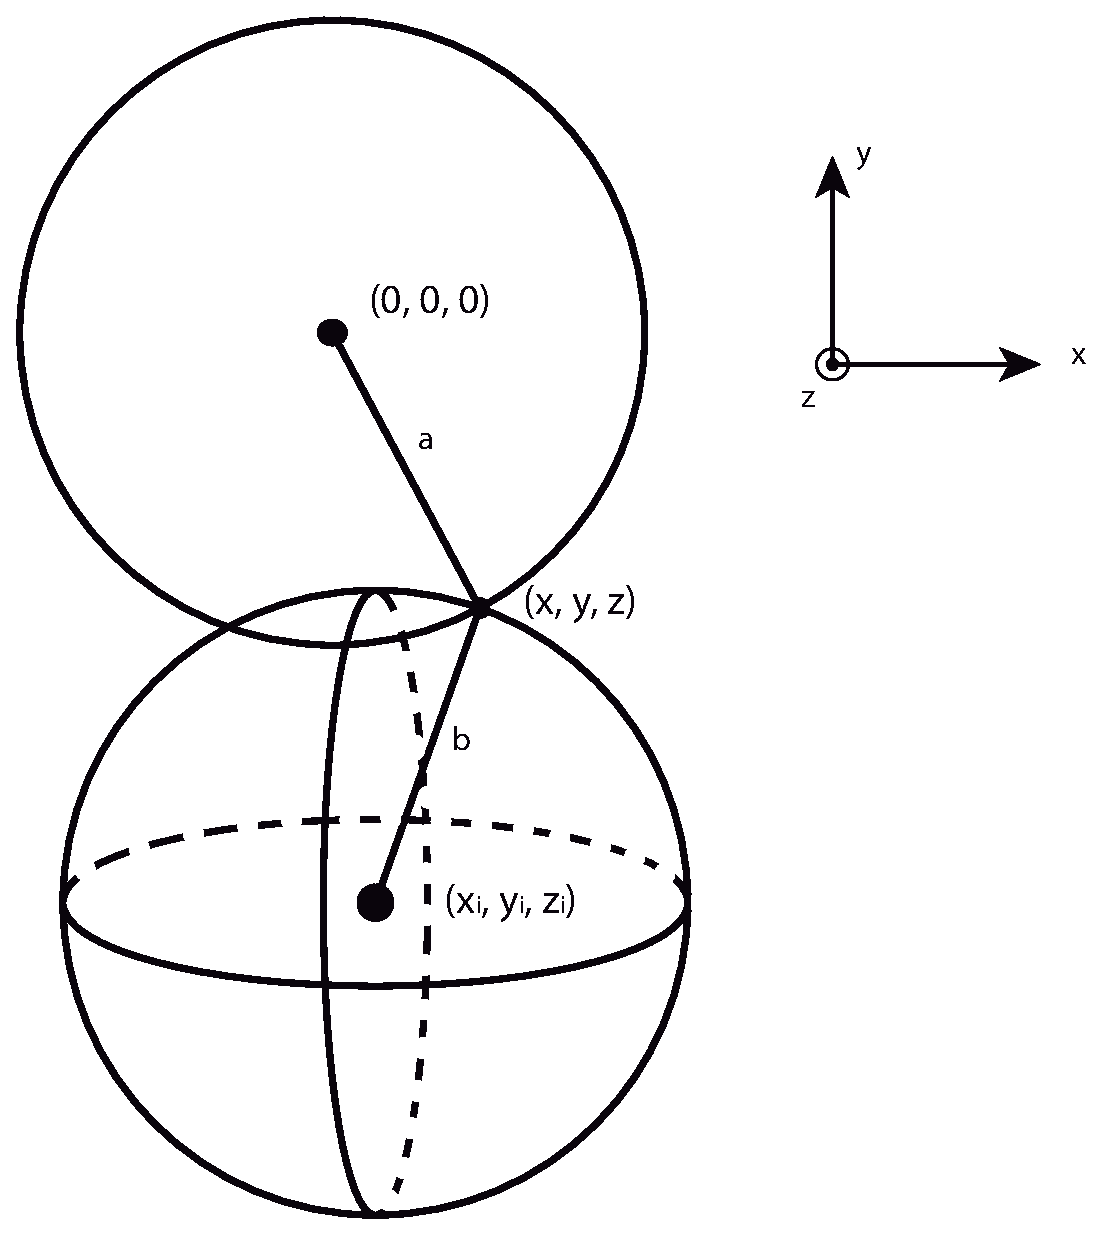
\includegraphics[width=8cm]{./sketch/calcul_angle}
\end{figure}

També es pot veure que, com ha d'estar connectat a la plataforma amb una distancia b mitjançant l'avantbraç, s'ha de complir la formula: \[(x-x_i)^2+(y-y_i)^2+(z-z_i)^2=b^2\]
Ara només cal resoldre el sistema d'equacions.

\[x^2 - 2xx_i + x_i^2 + y^2 - 2yy_i + y_i^2 + z_i^2 = b^2\]
\[-2xx_i - 2yy_i = \underbrace{b^2 - a^2 - x_i^2 - y_i^2 - z_i^2}_{n}\]
\[-2x_i\sqrt{a^2-y^2}=n+2yy_i\]
\[4a^2x_i^2-4y^2x_i^2=n^2+4yy_in+4y^2y_i^2\]
\[y^2(x_i^2+y_i^2)+y(y_in)+(\frac{n^2}{4}-a^2x_i^2)=0\]
\[y=\frac{-y_i\pm\sqrt{y_i^2n^2-4(x_i^2+y_i^2)(\frac{n^2}{4}-a^2x_i^2)}}{2(x_i^2+y_i^2)}\]
\[x=\pm\sqrt{a^2-y^2}\]
\[\textrm{Finalment, }\theta=atan(\frac{y}{x})\]

\subsection{Comprovació dels càlculs}

Per poder provar les nostres funcions sense trencar el robot, vam decidir fer una simulació en del Robot en Unity. La simulació es molt simple, Unity s'encarrega de dibuixar un esquema 3D del robot fent servir línies a partir de la posició desitjada de la plataforma i els angles del robot, calculats amb la nostra funció.

\begin{figure}[h!]
\centering
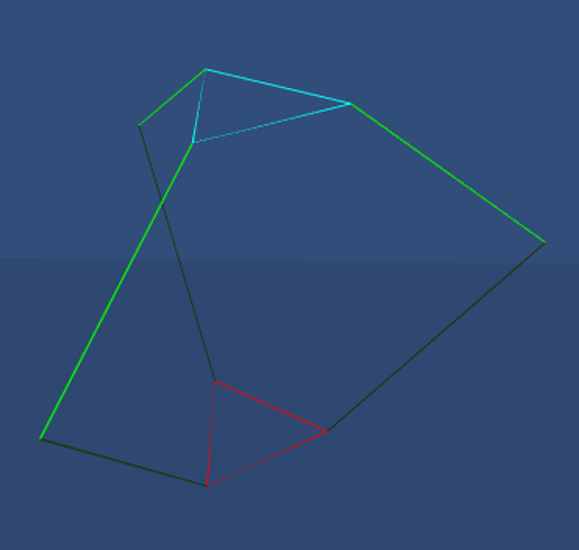
\includegraphics[width=7cm]{./images/simulacioRobot}
\end{figure}

Aquesta aplicació també es fa ver servir per determinar quin símbol s'ha de posar abans de les dos arrels. Per la primera arrel es va determinar que havia de anar acompanyada d'un signe negatiu només quan \(x_i\) és negatiu. La segona arrel només ha de ser negativa a partir de quan el ha d'estar completament cap a dalt. La condició exacta es: \(b^2-(y_i+a)^2<x_i^2+z_i^2\) 

\newpage
\subsection{Rang de treball}

Per calcular el rang de treball s'ha utilitzat la fórmula de l'apartat anterior i buscant una gran quantitat de punts, d'aquests els que donaven un resultat possible s'han agafat com a vàlids i els altres s'han descartat. Tot seguit s'han passat els punts a Matlab\textsuperscript{\textregistered} i s'ha generat la següent superfície.

\begin{figure}[h!]
\centering
\begin{minipage}{7cm}
\centering
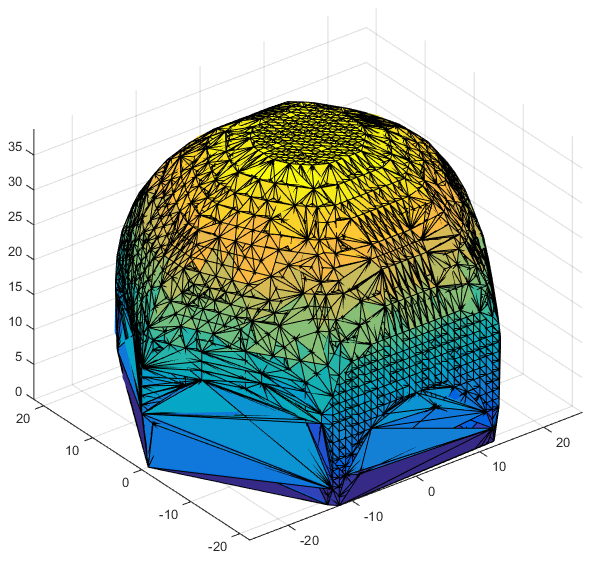
\includegraphics[width=7cm]{./images/rangTreball}
\end{minipage}
\\
\hfill
\begin{minipage}{7cm}
\centering
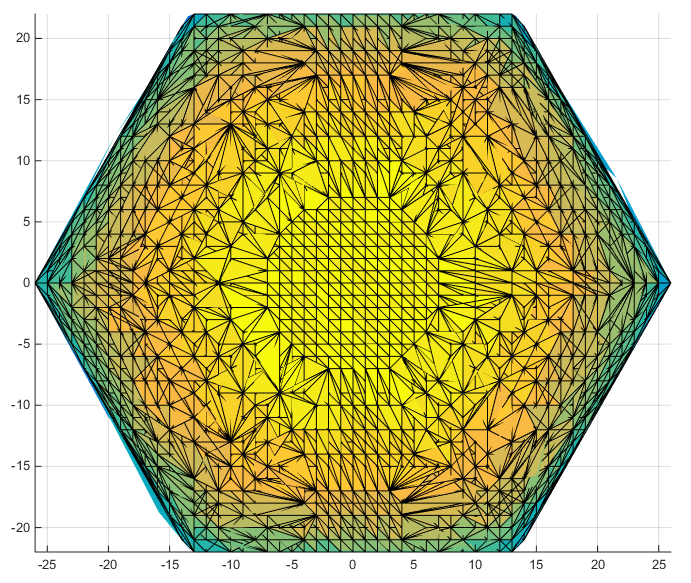
\includegraphics[width=7cm]{./images/rangTreball2}
\end{minipage}
\hfill
\begin{minipage}{7cm}
\centering
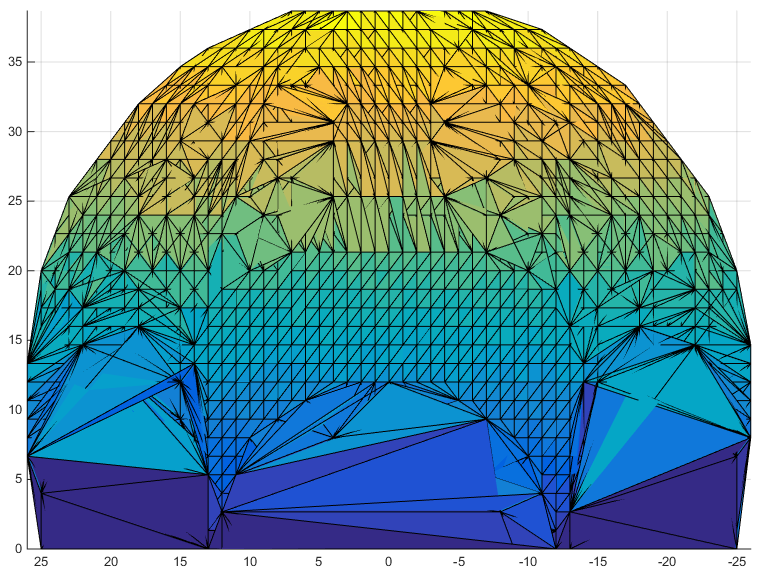
\includegraphics[width=7cm]{./images/rangTreball3}
\end{minipage}
\hfill
\end{figure}

Aquesta superfície esta calculada amb tots els punts possibles teòrics però el robot te moltes limitacions mecàniques que no es tenen en compte en aquest càlcul. Per exemple els paral·lelograms dels avantbraços no poden tenir un angle qualsevol, ja que les barres de metall xoquen contra les plaques de fusta del braç si l'angle es molt petit.

\clearpage
\subsection{Implementació en Matlab}

La implementació de Matlab té tres parts, dues per al càlcul dels angles de treball i la tercera per poder calcular el rang de treball del robot.

\subsubsection{Càlcul d'un angle}
\lstinputlisting[language=Matlab]{../Matlab/singleAngle.m}

\newpage
\subsubsection{Càlcul de tots els angles}
\lstinputlisting[language=Matlab]{../Matlab/setAngles.m}

\newpage
\subsubsection{Càlcul del rang de treball}
\lstinputlisting[language=Matlab]{../Matlab/calcWorkspace.m}
